\documentclass[12pt,a4paper,utf8x]{report}
\usepackage [frenchb]{babel}

%\usepackage{ucs}
\usepackage{pgfgantt}
\usepackage{graphicx}
\usepackage{caption}
\usepackage[utf8x]{inputenc}
\usepackage{multicol}
\usepackage{url} % Pour avoir de belles url
\usepackage {geometry}
%\usepackage {listings} %Pour mettre du code source 
\usepackage{verbatim}
\usepackage{lscape} % Pour pouvoir passer en paysage
\usepackage{listings}
\usepackage{geometry}
\usepackage{pdflscape}
\usepackage{colortbl}
\usepackage[strings]{underscore}
\geometry{left=2.5cm,right=2.5cm,vmargin=2cm}
\usepackage[pdftex,bookmarks = true,bookmarksnumbered = true,pdfpagemode = None,pdfstartview = FitH,pdfpagelayout = OneColumn,colorlinks=true,linkcolor=black,urlcolor=blue,citecolor=blue,pdfborder = {0 0 0}]{hyperref}


%chapitre---------------------------------------------------------------------
 
%%%% debut macro pour enlever le nom chapitre %%%%
\makeatletter
\def\@makechapterhead#1{%
  \vspace*{50\p@}%
  {\parindent \z@ \raggedright \normalfont
    \interlinepenalty\@M
    \ifnum \c@secnumdepth >\m@ne
        \Huge\bfseries \thechapter\quad
    \fi
    \Huge \bfseries #1\par\nobreak
    \vskip 40\p@
  }}

\def\@makeschapterhead#1{%
  \vspace*{50\p@}%
  {\parindent \z@ \raggedright
    \normalfont
    \interlinepenalty\@M
    \Huge \bfseries  #1\par\nobreak
    \vskip 40\p@
  }}
\makeatother
%%%% fin macro %%%% 

\begin{document}

\begin{titlepage}
\begin{flushright}
   	
\includegraphics[scale=0.30]{univorleans.png}\\ 
   	   	Département Informatique
\end{flushright}
\vspace{30mm}
\begin{center}
\huge{Rapport final \\Travaux d'étude et de recherche }\\
\vspace{8mm}
\large{Sujet : Android au pays des liseuses}\\
\vspace{3mm}
\large{Proposé et encadré par : Ollinger Nicolas}
\vspace{3mm}
\large{\\Réaliser par :}\\
\large{Fontorbe Jordan, Guillaume Arthur, Monediere Tristan, \\Rubagotti Joris}\\
\end{center}
\begin{figure}[b!]
\begin{flushright}
~~\\ ~~\\ ~~\\ ~~\\ ~~\\ ~~\\ ~~\\
\large{Année : 2012-2013}
\end{flushright}
\end{figure}
\end{titlepage}

\tableofcontents
\clearpage

\chapter{Résumé du projet}

Notre projet est proposé par M. OLLINGER et nous entraîne dans le monde des liseuses. Il consiste à étudier dans un premier temps les spécificités du déploiement d'Android sur une liseuse. Dans un second temps, d'émuler la plate-forme à l'aide d'une machine virtuelle sur un écran déporté sur un ordinateur. Tout le développement se concentrera sur la liseuse Sony PRS-T1 et son environnement Android fourni par notre chef de projet. 

%\section{Documentation}
%La première partie du projet a pour objectif de se documenter sur le sujet, c'est à dire la technologie du papier électronique et comment elle est mise en oeuvre au travers des différentes couches matérielles et logicielles.
%Cette partie va servir a la production de ce premier document de synthèse. 
%\section{Écriture du client RFB}
%Cette étape, a pour but de s'approprier les outils mis à notre disposition pour le développement. Il faudra dans un premier temps tester l'image de la liseuse. Puis mettre en oeuvre l'environnement de développement ltib de Freescale pour i.MX508. Il faut ensuite écrire un programme de test du framebuffer eink et ajouter un ioctl de mise à jour pour ensuite développer le support du gadget USB Ethernet au noyau. Il faut aussi ajouter ce module à l'image de test et une connexion via ssh. Il faut modifier DirectFB pour le support e-ink. Il faudra enfin modifier le protocole RFB pour supporter les mises à jour ioctl et mettre en oeuvre un client RFB pour la liseuse après avoir créé un serveur de gestion des mises à jour et effectuer des tests intensifs.
%\section{E-ink sous qemu via VNC}
%L'objectif de cette étape est de comprendre la gestion du framebuffer par l'émulateur qemu pour pouvoir y ajouter la gestion des ioctl. Dans un deuxième temps la compréhension de l'option VNC de qemu permettra l'ajout de l'extension RFB du client de la liseuse. Enfin des tests seront menés pour valider l'étape.
%\section{Liseuse Android sous qemu}
%Dans cette étape la compréhension des versions e-ink d'Android chez Freescale et Sony permettra la mise en place de cette pile dans l'émulateur. Cette étape sera testée à l'aide d'applications Sony. Enfin nous pourront écrire nos propres applications pour l'émulateur.
%\section{Simulateur d'écran E-ink}
%Cette dernière étape a pour objectif d'écrire un simulateur raisonnable d'écran e-ink. Celui-ci devra contenir une option de debug permettant d'afficher les zones de mise à jour. Le simulateur sera ensuite intégré à l'émulateur. Cette étape se terminera par des tests.
\section[Intruduction]{Introduction au domaine}


\subsection[E-Ink]{Technologie E-Ink}
\begin{frame}{Technologie E-Ink}
	%% A compléter par Arthur
\end{frame}


\subsection[Sony PRS-T1]{Liseuse Sony PRS-T1}

\begin{frame}{Caractéristiques principales} %% Liseuse en générale
	\begin{block}{Caractéristiques Sony PRS-T1}
		\begin{itemize}
			\item Processeur iMX508
			\item Écran E-Ink 6 pouces
			\item Résolution jusqu'à 16 niveaux de gris
			\item Interfaces USB
			\item WiFi
			\item Mémoire : 2Go (extensible par microSD)
		\end{itemize}
	\end{block}
\end{frame}

\begin{frame}{Processeur iMX508} %% partie iMX508
	\begin{block}{iMX508}
	\begin{itemize}
		\item{Développé par Freescale}
		\item{Architecture ARM Cortex A8}
		\item{Faible consommation d'énergie}
		\item{Bonnes performances}
		\item{Contrôleur d'écran intégré}
	\end{itemize}
	\end{block}
\end{frame}

\begin{frame}{Modules}
	\begin{block}{EPDC (Electrophoretic Display Controller)}
		\begin{itemize}
			\item{Dirige les signaux (waveform)}
			\item{Mise à jour partielle ou totale}
		\end{itemize}
	\end{block}
	\begin{block}{ePXP (enhanced Pixel Pipeline}
		\begin{itemize}
			\item Transparence
			\item Rotation d'image
			\item Agrandissement / Réduction d'image
		\end{itemize}
	\end{block}
\end{frame}

\begin{frame}{Architecture du processeur iMX508} %% Schéma
	\begin{figure}
		\begin{center}
			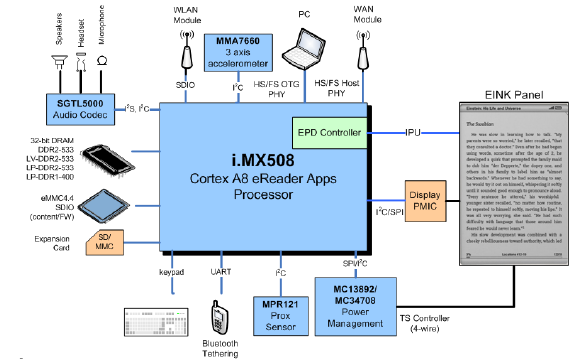
\includegraphics[scale=0.65]{iMX508.png}
		\end{center}
	\end{figure}
\end{frame}

\begin{frame}{Hack de la liseuse}
	\begin{block}{Mise à jour du firmware}
		\begin{itemize}
			\item Nécessite les clés privés de Sony
			\item Accès total à la liseuse
			\item Risque d'endommager la liseuse
		\end{itemize}
	\end{block}
	\begin{block}{Mode Recovery}
		\begin{itemize}
			\item Nécessite la recompilation du noyau
			\item Modifications sans risques
		\end{itemize}
	\end{block}
\end{frame}

\chapter{Analyse de l'existant}
\chapter{Besoins non fonctionnels}
\section{Hacks de la PRS-T1}

La PRS-T1 étant fermé, il nous est impossible dans sa configuration de base de pouvoir y ajouter la mise à jour 
de l'affichage depuis une machine hôte.
Plusieurs méthode existent pour débloquer la liseuse : 

\subsubsection{Mise a jour du firmware}

La méthode la plus répandues pour débloquer la liseuse consiste à faire une mise à jour du firmware.
La liseuse n'acceptant que les mises à jour signée par Sony. Les clefs privées de cette signature étant connues des hackers (elles sont stoquées dans la liseuse pour la vérification).

Plusieurs firmware modifié existe déjà pour mettre à jour la liseuse, c'est derniers débloque complètement la liseuse tout en gardant les logiciels Sony pré-installé.

Cette méthode dispose donc de plusieurs avantages : 
	\begin{itemize}
		\item permet un accès total a la liseuse (installation d'application Android, ...)
		\item on conserve les fonctions normale de la liseuse (logiciel de lecture Sony)
	\end{itemize}
Cependant le fait de modifier le firmware interne de la liseuse comporte certains risques : 
	\begin{itemize}
		\item risque de rendre la liseuse inutilisable
		\item perte de la garantie constructeur
	\end{itemize}

Étant donné que la PRS-T1 est un prêt de M. Ollinger cette méthode de hack comporte trop de risques.

\subsubsection{Utilisation du mode Recovery}

Une autre méthode de hack consiste à utiliser le mode recovery de la liseuse.
Ce mode permet normalement de récupérer la liseuse suite à un problème.
Pour entrer en mode recovery la liseuse a besoin d'un  système de fichier de récupération.
Ce dernier pouvant être situé sur une carte mémoire externe.

Cette méthode réduits les risques encouru lors de la manipulation car un simple redémarrage de la liseuse, 
suffit pour revenir au système de base.

les caractéristiques de cette méthodes sont  : 
%Les avantages de cette méthodes sont : 
\begin{itemize}
	\renewcommand{\labelitemi}{$\bullet$}
	\item Avantages : 
	\begin{itemize}
		\item risque minime pour la liseuse
		\item permet des modifications importante (car on fait nous même le système à partir des sources du noyau fournit par Sony)%un peu long non ?
	\end{itemize}
	\item désavantages : 
		\begin{itemize}
			\item nécessite un pc hôte pour la mise en place du système (nécessitent de compiler le noyau)
			\item On repart de zéro donc on n'a pas accès aux application sony (pour la lecture d'Ebook notamment)
			\item nécessite beaucoup de travail car on repart avec uniquement le noyau.
		\end{itemize}
\end{itemize}
\section{Risque}
\subsection{Les Waveformes}
	Le driver permet de redéfinir les fonctions de waveforme du contrôleur.
Cependant le bon fonctionnement des écrans E-Ink dépend fortement de ces fonctions, modifier ces fonctions peut donc entraîner dans le meilleur des cas une différence entre la représentation virtuelle de l'affichage et ce que va réellement afficher l'écran, dans le pire cas cela peu endommager de manière définitive l'écran de la liseuse.

\section{Tests}

La spécificité des liseuses venant de leur écran il faut faire attention a respecter au maximum le comportement de ce dernier pour faire un environnement de développement dédié aux liseuses.

\subsubsection{Taux de rafraîchissement}

Les écrans E-Ink ayant un taux de rafraîchissement assez bas il devient nécessaire de veiller à ne pas le réduire d'avantage.
Pour cela Il va falloir mettre en place un test comparatif entre le rafraîchissement de la liseuse seule et le rafraîchissement avec un ordinateur hôte via VNC.

\subsubsection{Update bloquante}

De la même manière l'ordinateur hôte ne doit pas se comporter de la meme manière qu'avec un écran classique. En effet il serait très facile pour l'hôte de surcharger complètement l'écran en faisant des mises à jour de l'affichage comme il le ferait avec un écran classique. %a véifier un peu tordu
\chapter{Besoins fonctionnels}

Comme énoncé dans le chapitre 1 de ce document, le but du projet est la réalisation d'un émulateur d'une liseuse avec un écran virtuel fonctionnant comme un écran E-Ink directement sur notre machine ayant pour système d'exploitation Linux. La réalisation de ce projet se découpe en plusieurs parties à réaliser dans un ordre strict afin d'aboutir au résultat final souhaité. Ce plan nous a été proposé par notre encadrant de projet M. OLLINGER. N'ayant pas encore eu le temps de tester les points suivants il se peut que certains des éléments ont été mal interprétés d'où la présence possible d'erreurs. D'autres points peuvent aussi manquer de détails.

\section{Conception d'un client RFB pour la liseuse}

Dans un premier temps il nous faut concevoir un prototype de client permettant de mettre à jour l'écran de la liseuse de test via notre ordinateur.

\subsection{DirectFB}
Pour réaliser cela, il nous a été proposé de travailler avec DirectFB. C'est une bibliothèque libre qui fournit à la fois un accès aux composants matériels graphiques (accélération graphique) ainsi qu'aux périphériques d'entrées, et un systèmes de gestion de fenêtres intégrées avec support de la transparence et de calques multiples. Tout ceci à travers l'interface framebuffer de Linux. Nous devons ajouter la gestion des écrans E-Ink dans DirectFB. 
 
\subsection{Client RFB}
Lorsque DirectFB est prêt à être employé, on travaille ensuite sur le protocole RFB (Remote FrameBuffer) qui est un simple protocole permettant des accès à distance à des interfaces graphiques d'utilisateur. On doit ajouter la gestion des mises à jour de l'affichage pour les écrans de type E-Ink via ioctl. De tous ces éléments, on peut ainsi concevoir un client RFB interagissant sur la liseuse et la conception d'un serveur gérant les mises à jour.
\\Les tests consisteront à essayer de produire des changements d'affichage sur la liseuse grâce à des demandes précises envoyées via l'ordinateur de test et transmis par le serveur de mise à jour. 

\newpage

\section{E-Ink QEMU via VNC}

Dans un second temps, on développe la base de l'émulateur, c'est à dire la mise en place d'une machine virtuelle pouvant reproduire les actions nécessaires au fonctionnement d'un écran E-Ink. Pour réaliser cela, nous travaillons sur QEMU qui permet l'émulation de processeur et de machine virtuelle permettant l'exécution de système d'exploitation. On ajoute la gestion des ioctl à QEMU. Ensuite il faut ajouter à l'option VNC de QEMU l'extension RFB du client de la liseuse.
\\Le test consiste à vérifier si depuis une machine virtuelle QEMU utilisant l'image du noyau Linux de la liseuse de test, on peut via VNC interagir avec la liseuse. 


\section{Liseuse Android sous QEMU}

Après la création de la base de l'émulateur, on intègre à celui-ci un système d'exploitation Android conçu pour fonctionner sur une liseuse. Dans notre cas ça sera la version d'Android présente sur notre liseuse de test SONY PRS-T1.
Pour les tests, on lance l'émulateur muni d'Android et on test le fonctionnement des applications SONY fournies de base avec le système d'exploitation.

\section{Simulation d'écran E-Ink}

Pour finir le développement de l'émulateur, on développe un simulateur d'écran E-Ink reproduisant virtuellement le comportement de celui-ci en y ajoutant des fonctionnalités facilitant les tests telles que choisir une zone précise à mettre à jour sur un écran (utile au debug). Ensuite on intègre celui-ci dans notre émulateur.
\\Les tests consisteraient à réaliser des mini-applications, les lancer sur l'émulateur et vérifier les réactions de notre écran virtuel.


\chapter{Résultats de tests}
\begin{landscape}
\chapter{Planning}

\begin{figure}[h!]
\begin{center}

\begin{ganttchart}[y unit title=0.4cm,
y unit chart=0.5cm,
vgrid,hgrid, 
title label anchor/.style={below=-1.6ex},
title left shift=.05,
title right shift=-.05,
title height=1,
bar/.style={fill=gray!50},
incomplete/.style={fill=cyan},
progress label text={},
bar height=0.7,
group right shift=0,
group top shift=.6,
group height=.3,
group peaks={}{}{.2}]{32}
%labels
\gantttitle{Planning}{32} \\
\gantttitle{Février}{8} 
\gantttitle{Mars}{8} 
\gantttitle{Avril}{8} 
\gantttitle{Mai}{8} \\
%tasks
\ganttbar[bar/.style={fill=green, rounded corners=3pt}]{Recherche Doc}{1}{8} \\
\ganttbar[bar/.style={fill=blue, rounded corners=3pt}]{Réunion}{9}{10} \\
\ganttbar[progress=90,bar/.style={fill=orange, rounded corners=3pt}]{Dev DirectFB}{11}{17} \\
\ganttbar[progress=90,bar/.style={fill=orange, rounded corners=3pt}]{Dev Client RFB}{11}{17} \\
\ganttbar[progress=90,bar/.style={fill=orange, rounded corners=3pt}]{Dev Serveur Update}{11}{17} \\
\ganttbar[progress=90,bar/.style={fill=orange, rounded corners=3pt}]{Dev QEMU et VNC}{17}{21} \\
\ganttbar[progress=90,bar/.style={fill=orange, rounded corners=3pt}]{Dev QEMU Liseuse SONY}{18}{22} \\
\ganttbar[progress=90,bar/.style={fill=orange, rounded corners=3pt}]{Dev Simulation Ecran}{23}{27} \\
\ganttbar[bar/.style={fill=yellow, rounded corners=3pt}]{Finalisation}{28}{31}
\end{ganttchart}
\vspace{-0.5cm}
\end{center}
\hspace{7.3cm} \noindent \begin{tabular}{l}
	 \rowcolor{green} \\  
\end{tabular}
Recherche documentaire

\hspace{7.3cm} \noindent \begin{tabular}{l}
     \rowcolor{blue} \\  
\end{tabular}
Réunion du groupe pour mettre en commun tous les éléments et répartir les taches 

\hspace{7.3cm} \noindent \begin{tabular}{l}
     \rowcolor{orange} \\  
\end{tabular}
Phase de développement

\hspace{7.3cm} \noindent \begin{tabular}{l}
     \rowcolor{cyan} \\  
\end{tabular}
Phase de test

\hspace{7.3cm} \noindent \begin{tabular}{l}
     \rowcolor{yellow} \\  
\end{tabular}
Finalisation du TER \\
\caption{Planning de réalisation du projet}
\end{figure}
\end{landscape}
\chapter{État final de développement}

L'avancement actuel du projet, permet : 
\begin{itemize}
	\item d'établir une connexion Ethernet entre le PC hôte et la liseuse
	\item de modifier l'affichage de l'écran E-Ink
\end{itemize}

La mise en place de la connexion Ethernet se fait grâce aux modifications effectuées sur le système de fichiers monté par la liseuse.

% 1 : l'image de la liseuse
%ethernet
	%connection de l'interface reseau eth1 
\section{Fonctionnalités de l'image} %a changer

\subsection{La connexion Ethernet}
La liseuse ne disposant que d'un port USB il faut passer par un module chargeable pour émuler une connexion Ethernet sur ce port.
Ce module est le gadget Ethernet d'Android.
Le réseau établi entre la liseuse et le PC est défini statiquement, de plus les adresses MAC des cartes émulées sont fixées par le module.

%capture d'ecran ifconfig
\begin{figure}[]
	\begin{center}
	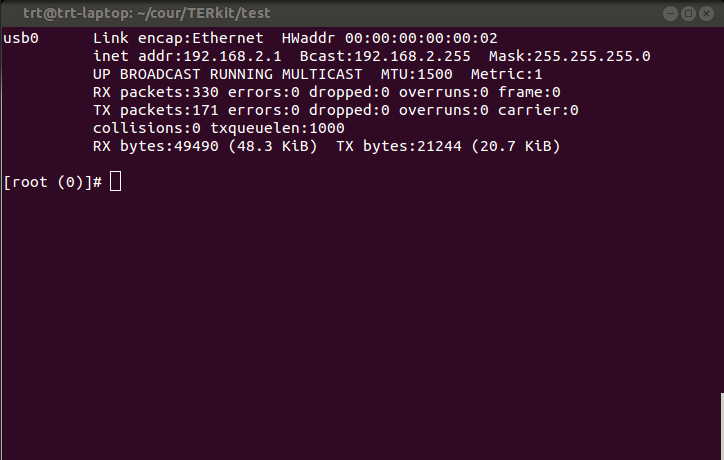
\includegraphics[scale=0.5]{capt_prs_ifconfig.png}	
	\end{center}
	\caption{Configuration réseau de la liseuse}
\end{figure}

\begin{figure}[]
	\begin{center}
		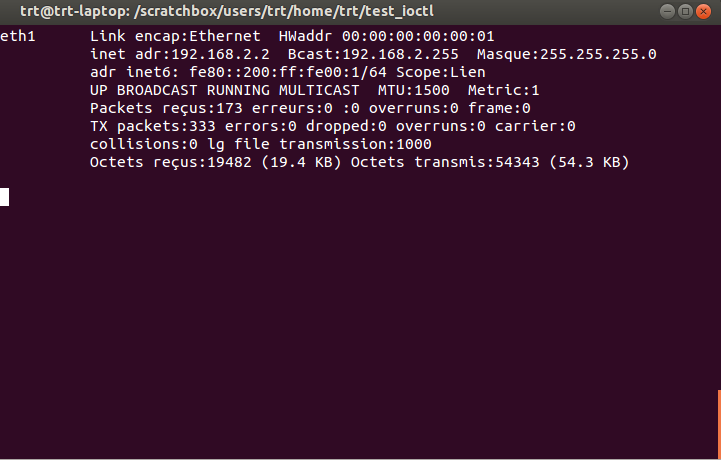
\includegraphics[scale=0.5]{capt_pc_ifconfig.png}
	\end{center}
	\caption{configuration réseau du PC}
\end{figure}
\clearpage
%dropbear
\subsection{L'ajout de dropbear}
Pour des raisons pratiques nous avons ajouté à la liseuse la gestion du protocole SSH, afin de pouvoir lancer facilement des commandes sur la liseuse, mais aussi de faciliter la copie de fichiers.
%a voir ci c'est util
L'utilisation de dropbear est pratiquement identique à celle du SSH que l'on peut trouver sur un système Linux. De légères différences subsistes si une connexion en SSH de la liseuse au PC hôte car les commandes ne sont pas nommées comme sur un système classique. Pour démarrer le serveur Dropbear (SSH) la commande est la suivante : 

\begin{lstlisting}
dropbear start
\end{lstlisting}

Normalement dropbear est démarré au lancement de la Liseuse en mode Recovery. De plus si une connection ssh veut être initialisé de la liseuse, il faut lancer la commande suivante :

\begin{lstlisting}
dhclient [nom-hote]@[IP-hote]
\end{lstlisting}



\section{Programme d'affichage}

La modification de l'écran E-Ink peut se faire de deux manières, soit en envoyant les commandes directement au driver (en utilisant les ioctl), soit en passant par une librairie graphique (ici DirectFB).

\subsection{Affichage via ioctl}

Le programme de test d'affichage via ioctl permet d'envoyer un buffer d'affichage directement dans le framebuffer du driver EPDC.
Ici ce buffer est constitué de pixels aléatoire : 
%capture d'écran get_temp
	
	\begin{figure}[h!]
		\begin{center}
			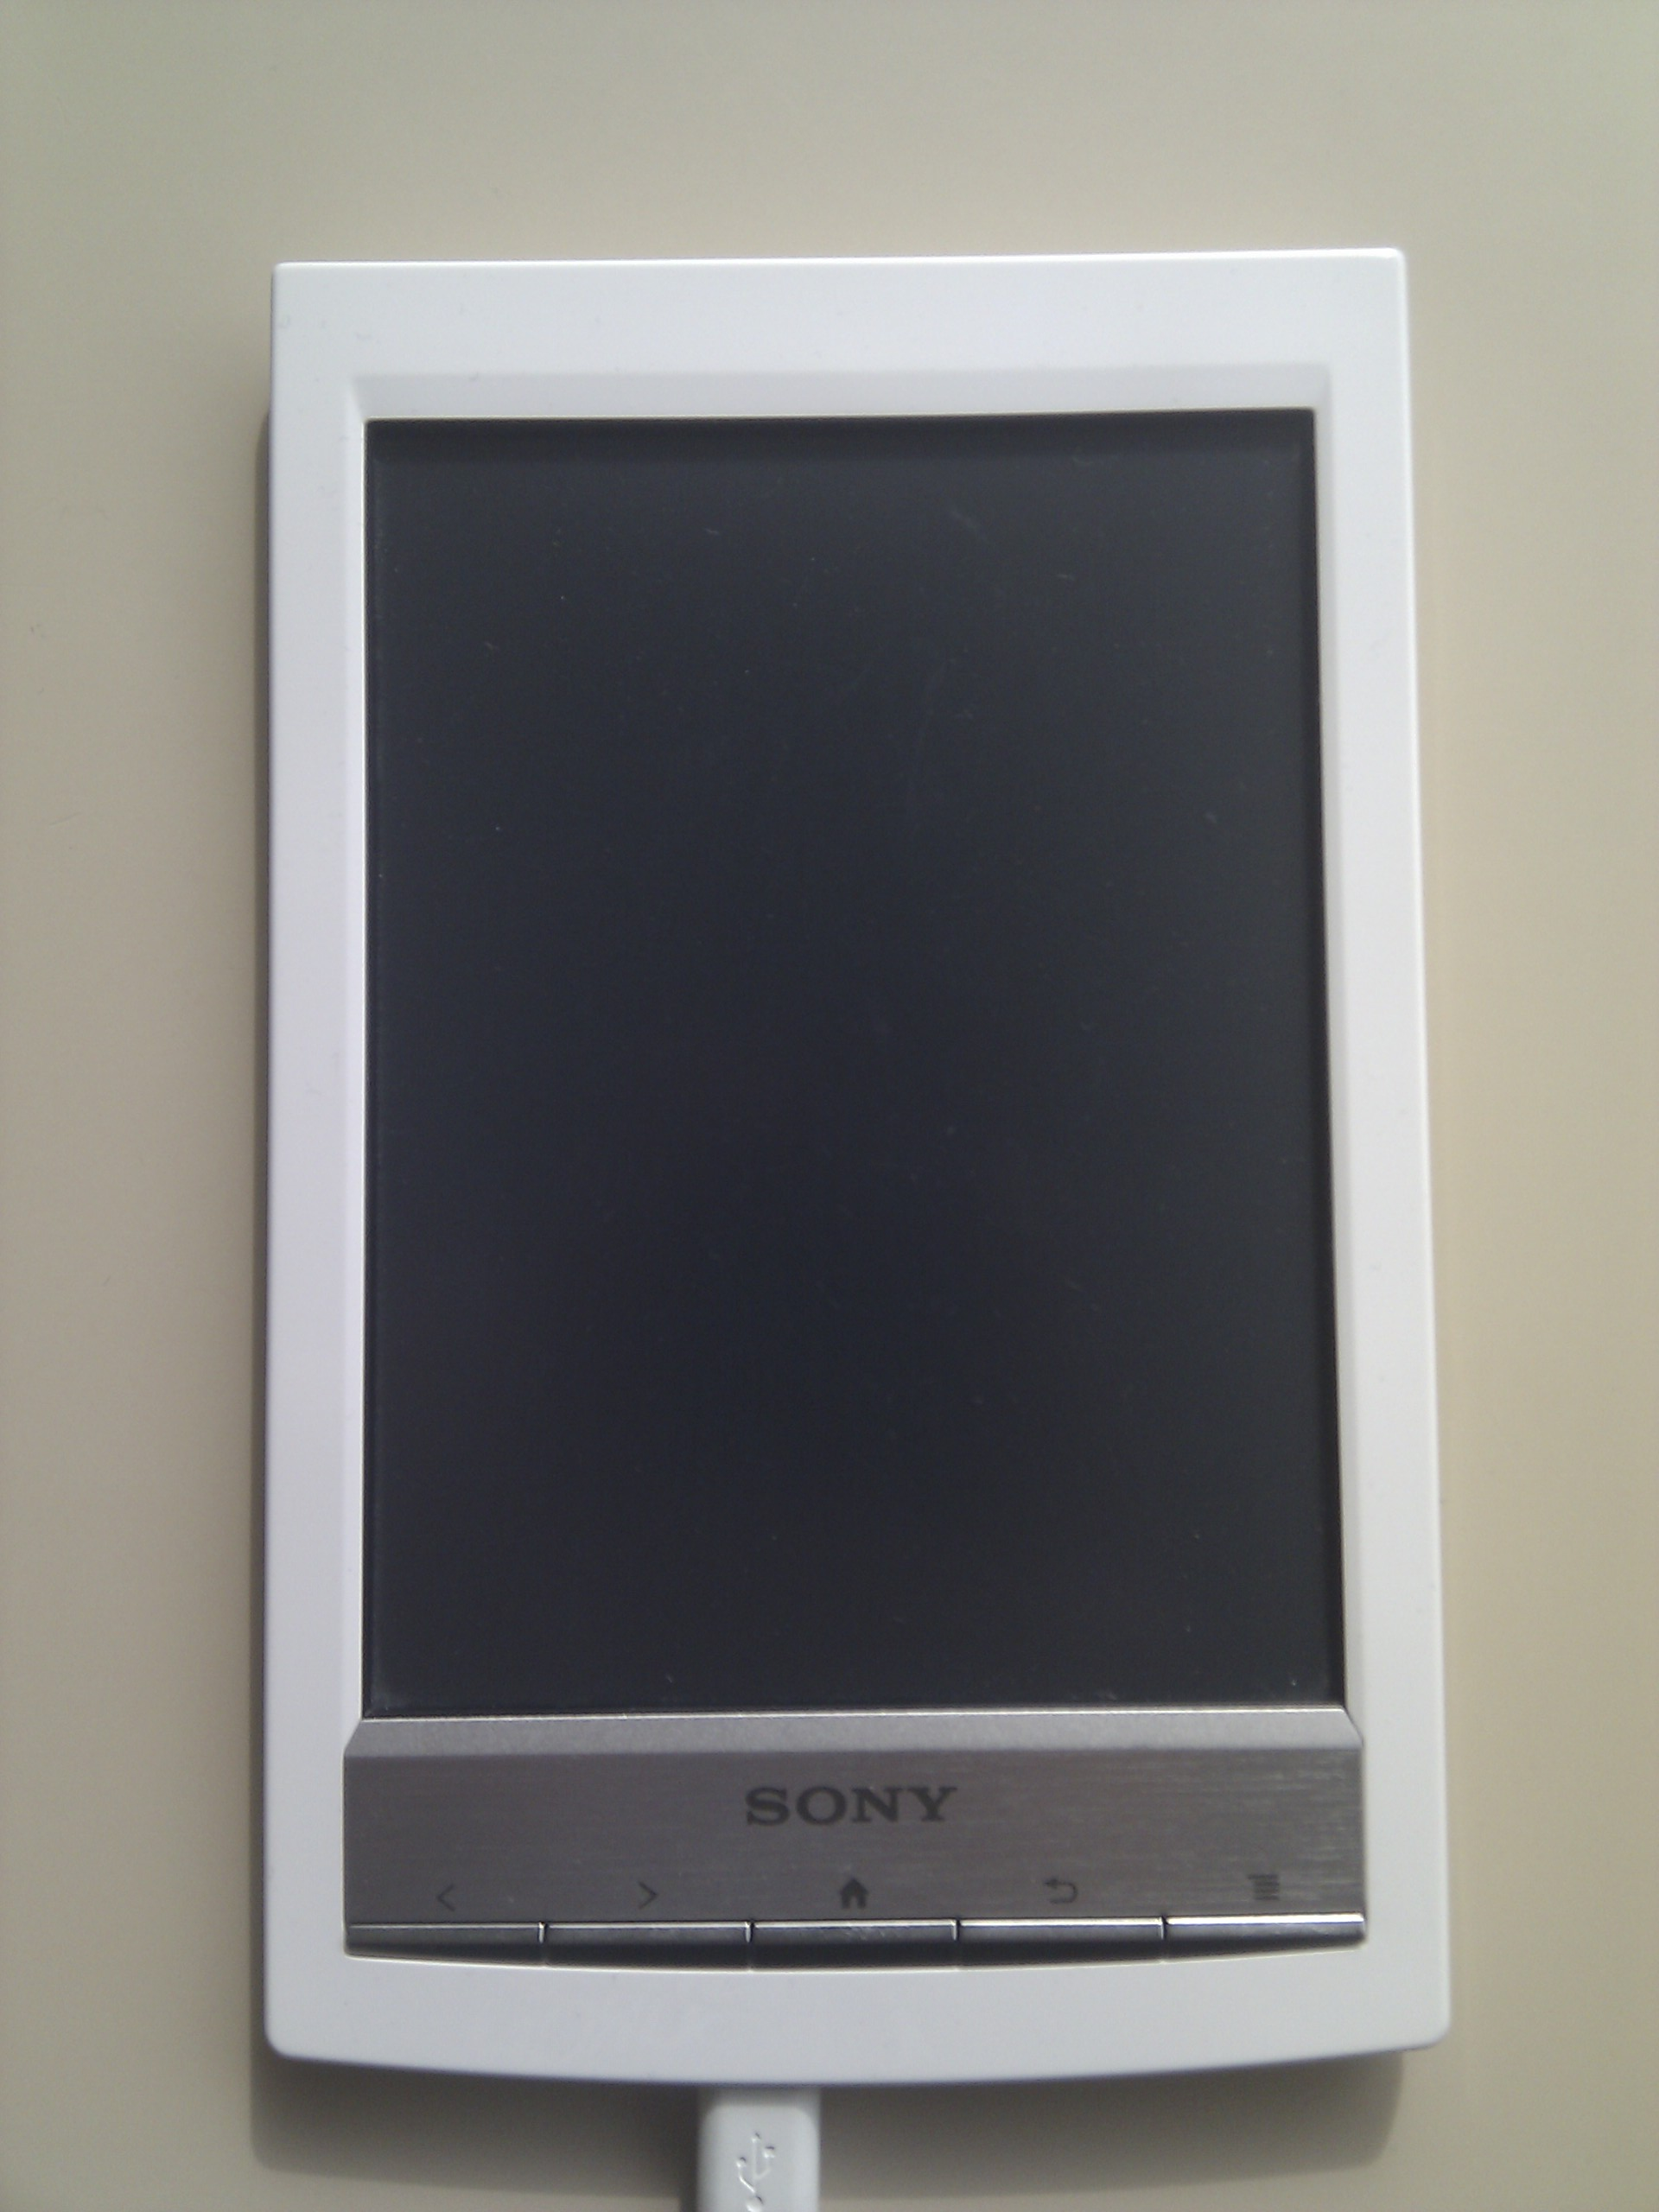
\includegraphics[scale=0.15]{screen_get_temp.jpg}
			 \caption{Modification de l'affichage en utilisant les ioctl}
		\end{center}
	\end{figure}
\subsection{Affichage via DirectFB}

Le programme d'affichage via Librairie graphique génère le framebuffer en utilisant les primitives de DirectFB.
Le programme de test dessine ici 10 lignes avec points d'arrivé aléatoire.

	\begin{figure}[h!]
		\begin{center}
			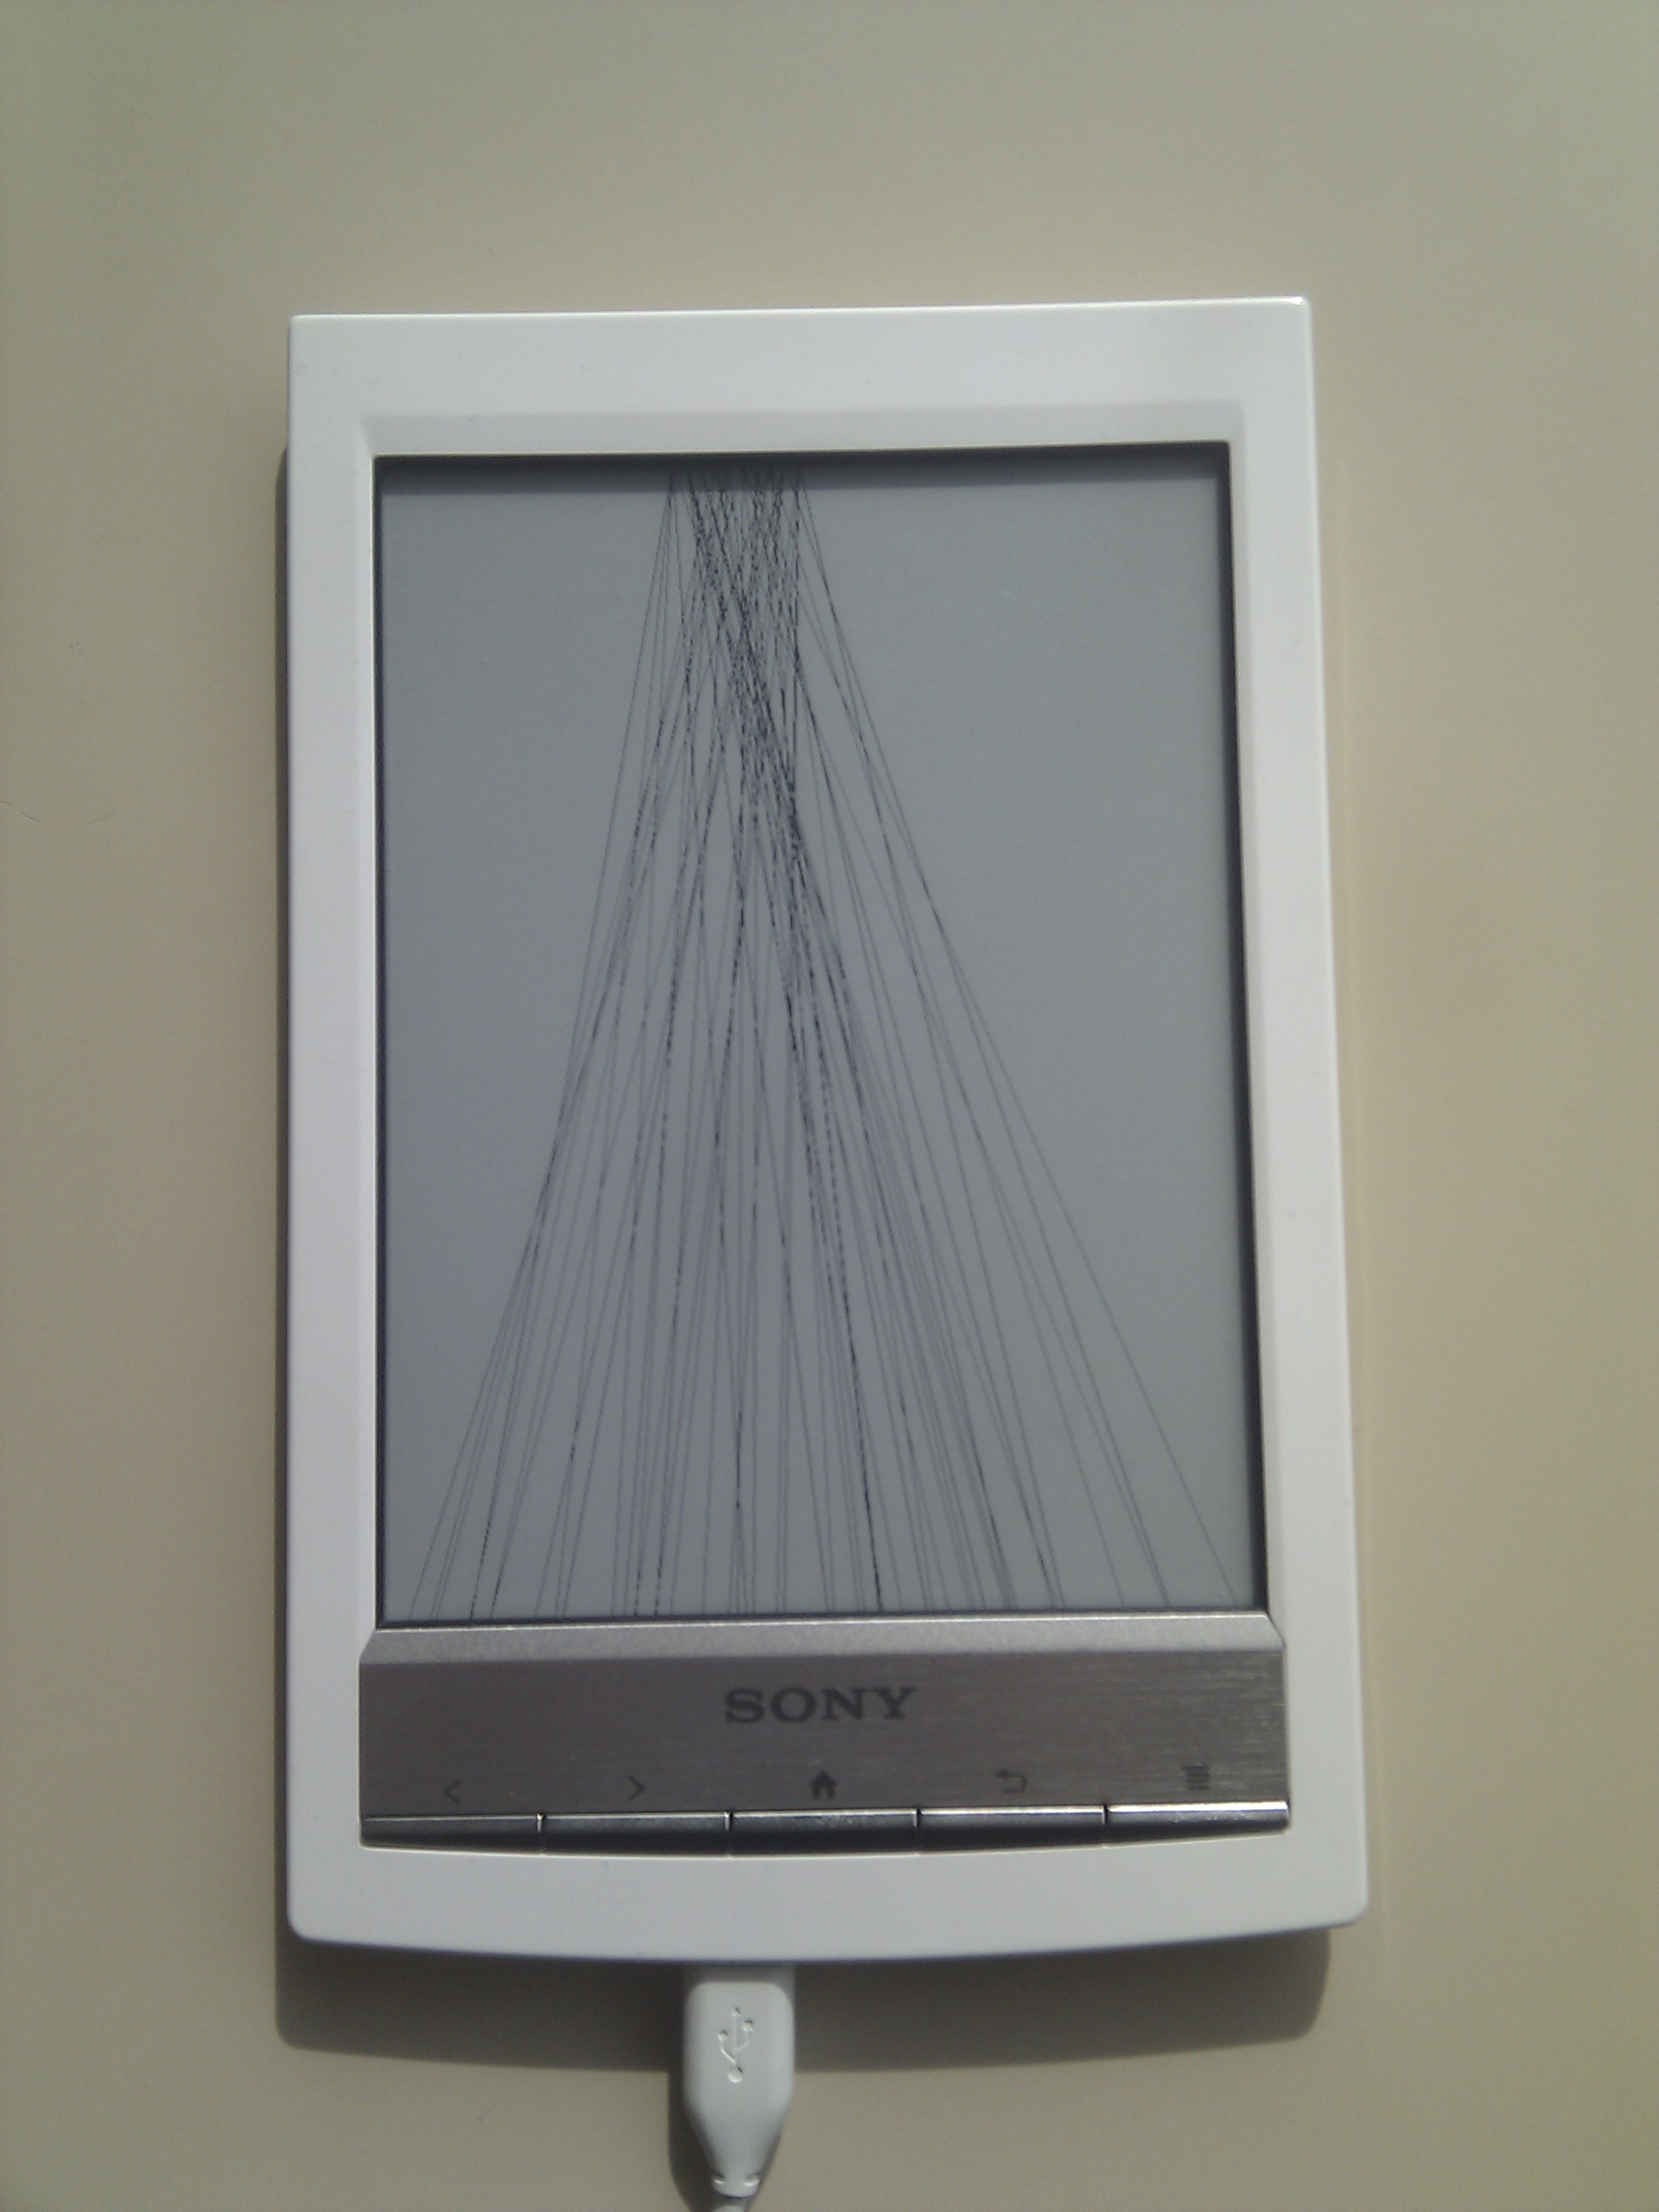
\includegraphics[scale=0.15]{screen_direct.jpg}
			\caption{modification de l'affichage en utilisant DirectFB}
		\end{center}
	\end{figure}

%capture direct
% 2 : programme d'affichage
%exemple de fonctionnement

\chapter{Architecture du projet}

\section{L'image du mode recovery}

\subsection{L'image de base}
Le mode Recovery se base sur le kernel Linux 2.6.35.3 qui est contenu dans une ROM interne à la liseuse (il est donc inaccessible). Le système de fichier est compris dans un fichier image contenu lui sur la carte SD, ce fichier peut être modifié depuis l'extérieur.

L'image fournie par défaut pour le mode Recovery, contient : 
\begin{itemize}
	\item un exécutable Busybox \\
		qui permet l'accès aux commandes usuelles Linux dans les systèmes embarqués
	\item un serveur DHCP
	\item un démon telnet
	%peut etre a mettre dans la partie du rapport intermediaire
	\item un accès au port USB en mode série (via le module g_serial)
\end{itemize}


Le système de fichier du mode Recovery est en lecture seule, seuls les dossiers suivant sont accessibles en lecture / écriture : 
\begin{itemize}
	\item /etc
	\item /initrd/mnt/sd
	\item /tmp
\end{itemize}

Pour modifier le système de fichier racine il faut passer par un PC hôte.

\subsection{L'image finale}

L'image finale ajoute les fonctionnalités suivante à l'image : 
	\begin{itemize}
		\item un accès au port USB par connexion Ethernet
		\item le support du protocole SSH
		\item la librairie DirectFB
	\end{itemize}

Plusieurs fonctionnalités devenues inutiles ont été désactivées :
\begin{itemize}
	\item Le serveur DHCP : \\
		il est peu utile d'avoir un support DHCP alors que le PC hôte et la liseuse 
		ont un réseau pour eux seuls.
		%peut etre rajouté le fait qu'il sont en plus défini statiquement ??
	\item Le démon telnet : \\
		la gestion du protocole telnet est devenu inutile et peu pratique (la copie de fichier
		 n'étant pas géré par exemple), depuis l'ajout du support du protocole SSH.
\end{itemize}

L'émulation d'un lien Ethernet sur le port USB de la liseuse se fait via le module g_ether.
%a verifier si c'est pas déjà dis avant
Ce module est situé comme les autres modules dans :
	\begin{lstlisting}
	/lib/modules/2.6.35.3/kernel/drivers/usb/gadget
	\end{lstlisting}

Le support du protocole SSH se fait via l'exécutable Dropbear situé dans : 
	\begin{lstlisting}
	/bin
	\end{lstlisting}

Les fichiers concernant la librairie DirectFB se situe dans le dossier /usr/local/lib.
Pour pouvoir lancer une exécutable utilisant DirectFB il faut vérifier que ce dossier soit bien inclus dans la variable d'environnement LD_LIBRARY_PATH, cette variable est définie dans le script rc.local.
\section{La mise en place de l'affichage}
%architecture pour affichage via directfb

L'affichage de la liseuse se fait grâce aux modules suivant : 
\begin{itemize}
	\item le driver mxc_epdc
	\item DirectFB
\end{itemize}~\\

Le driver se charge de faire les optimisations pour pallier au problème de réactivité de l'écran (via les tables LuT notamment), ainsi que l'application des waveforms pour l'affichage sur l'écran.\\
Le driver fournit des ioctl pour permettre l'exécution des fonctionnalités du driver depuis l'espace utilisateur.~\\~\\
%verifier si c'est pas deja dis plus tot dans le rapport
DirectFB implémente des primitives graphiques, comme le traçage de ligne. Ces dernières permettent de faire une abstraction sur le format du framebuffer.

Voici un schéma modulaire de l'application utilisant DirectFB : 

\begin{figure}[h!]
	\begin{center}	
		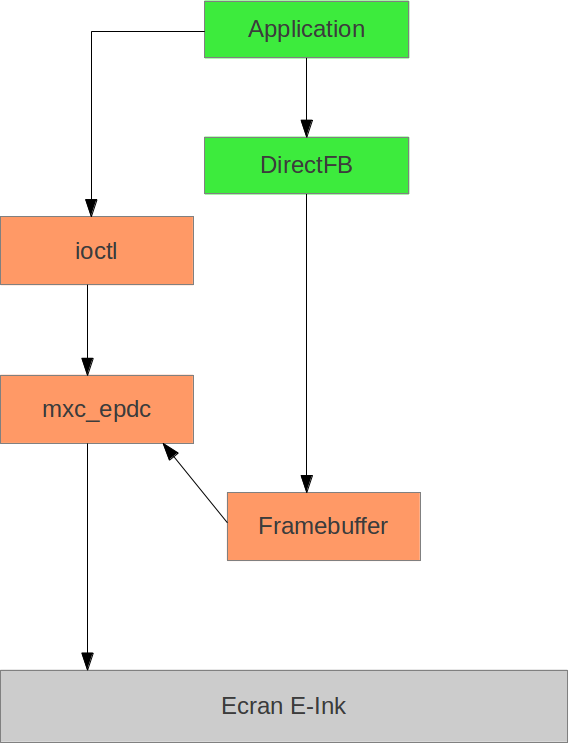
\includegraphics[scale=0.5]{schema_direct_fb.png}
		\caption{Architecture modulaire de l'application}
	\end{center}
\end{figure}

Dans l'état d'avancement actuel du projet, le programme met à jour le framebuffer via DirectFB et fait un appel ioctl au driver qui actualise l'écran en fonction du buffer. 
% application => directfb => framebuffer 				=> affichage
%						 => ioctl 	=> driver epdc   ||


%explication du fonctionnement 

% description de chaque module 
% directfb : abstraction du driver d'affichage
% ioctl : appel de la maj driver
%
%framebuffer
\chapter{Développement effectué}

Dans ce chapitre nous présenterons les différents moyens nous ayant permis d'obtenir le résultat final présenté dans le chapitre "État final de développement".\\ 
Dans un premier temps nous parlerons de la mise en place du module permettant une communication Ethernet via le port USB de la liseuse. Dans un second temps nous présenterons la mise en place de Dropbear (SSH) sur la liseuse facilitant les accès réseaux sur la machine de test et permettant ainsi la copie de fichier du PC hôte vers la liseuse. Ensuite nous présenterons les étapes nécessaires à la compilation de DirectFB. Et pour finir nous détaillerons des exemples de code permettant la modification de l'affichage de la liseuse avec DirectFB ou les ioctl.

\section{Module g_ether}
\subsection{Configuration}

Les commandes suivantes ont été testées sur deux systèmes d'exploitation Linux différents : 
\begin{itemize}

\item Ubuntu 12.04 x64 
\item Archlinux x64(Version du kernel : 3.8.*-*-ARCH)

\end{itemize}


Pour la cross-compilation, on a utilisé, dans cette section, le compilateur GCC 4.4.3 fourni avec l'android NDK. Pour la bonne utilisation de celui-ci et non le GCC présent sur notre système, on configure la variable PATH avec le chemin d'accès au GCC du NDK et on indique d'autres éléments et d'autres variables d'environnement pour obtenir la bonne compilation :

\begin{lstlisting}
# Attention le PATH suivant peut etre different sur certain systeme
export PATH=[PATH_to_ndk]/linux-x86/toolchain/arm-eabi-4.4.3/bin 
export CROSS_COMPILE=arm-eabi-
export SUBARCH=arm
export ARCH=arm
\end{lstlisting}

Pour la configuration du kernel(2.6.35.3) pouvant être utilisé sur la liseuse, on a employé le contenu de l'archive config.gz que l'on a décompressé dans le répertoire de ce kernel puis on a effectué la commande "make menuconfig". Voici la procédure employée :

\begin{lstlisting}
zcat [PATH_to_terkit]/nopid/livedata/config.gz \
[PATH_to_terkit]/sony/linux-2.6.35.3/.config

cd [PATH_to_terkit]/sony/linux-2.6.35.3/
make menuconfig
\end{lstlisting}

Suite à la commande "make", une fenêtre s'ouvre dans le terminal qui permet de sélectionner certaines fonctionnalités pour le kernel. Pour l'option à éditer, il faut se rendre dans le menu suivant: \\
Device drivers $>$ usb support $>$ usb gadget support \\
L'option à modifier dans la page est Ethernet gadget en l'activant ($<$M$>$) et laisser l'option RNDIS support en valeur par default ([*]).\\

Au cours de la phase suivante, on a obtenu une erreur lors de la compilation du kernel donc pour éviter cette erreur, on a modifié la ligne 135 du fichier fs/nfs/nfsroot.c :

\begin{lstlisting}
# on modifie la ligne 135 :
static const match_table_t tokens __initconst = {
# par la ligne suivante :
static const match_table_t tokens /*__initconst */ = { 
\end{lstlisting} 

Ensuite on a compilé les modifications avec la commande suivante :

\begin{lstlisting}
make modules
\end{lstlisting}

Pour finir on a copié le fichier g_ether.ko dans le système de fichier de la liseuse dans le répertoire suivant : /lib/modules/[version]/kernel/drivers/usb/gadget
 
\subsection{Installation du modules}

Initialement la liseuse possède un module g_serial, qui après quelques tests, rentrait en conflit avec le module g_ether installé. On a désactivé le module g_serial puis on  a lancé le module g_ether. Pour réaliser cela au démarrage de la liseuse, on a édité le fichier "/etc/rc.d/rc.local" en ajoutant les lignes suivantes à la fin : 

\begin{lstlisting}
echo "modprobe -r g_serial" > /initrd/mnt/sd/test/log
#desactivation de g_serial
modprobe -r g_serial 2>> /initrd/mnt/sd/test/log
echo "modprobe g_ether" >> /initrd/mnt/sd/test/log
#activation de g_ether
modprobe g_ether host_addr=00:00:00:00:00:01 \
dev_addr=00:00:00:00:00:02 2>> /initrd/mnt/sd/test/log
#on demarre l'interface
ifconfig usb0 up
ifconfig usb0 192.168.2.1
\end{lstlisting}		

En utilisant la sortie standard vers un fichier de log, on a pu observer la présence d'erreurs lors de l'exécution de ces différentes commandes. En effet à cause de la désactivation du module g_serial, il n'était plus possible de se connecter à la liseuse si une erreur était présente lors du chargement du module g_ether.
Les options host_addr et dev_addr permettent à la liseuse d'affecter son adresse MAC mais aussi celle de la machine hôte sur laquelle elle est connectée (host), cela permet de ne pas avoir à refaire la configuration réseau à chaque branchement en USB.	\\
	%connection depuis le pc
	Pour se connecter depuis le pc hôte on a pensé à vérifier que le module usbnet était bien activé (normalement automatique sur les systèmes récents).	
	Une interface réseau devrait apparaître et il faut la configurer sur le sous-réseau 192.168.2.0/24 (la liseuse est configurée sur l'adresse 192.168.2.1/24)

\newpage

\section{Informations de configuration}

Avant d'expliquer les différentes procédures de cross-compilation pour les différents besoins du projet, voici une liste d'informations sur les paramètres des fichiers "configure" ou de variables d'environnement rencontrées :

\begin{lstlisting}
# Variables d'environnements ajoutees
 PATH => chemin vers un repertoire qui contiennent des
 executables que vous souhaitez pouvoir lancer sans
 indiquer leur repertoire.
 CC => cross-compilateur employe (gcc)
 CXX => compilateur g++
 CPP => compilateur cpp
 AR => archivage et indexation
 RANLIB => indexation
 LD => linker
 STRIP => supprime la table des symboles
 CCFLAGS => precise l'architecture de sortie au compilateur

# Parametres generaux
  
  --build=BUILD   indique l'architecture sur laquelle
                  la compilation a lieu
  --host=HOST     indique l'architecture du systeme ou
                  sera lance le programme   
  --target=TARGET indique l'architecture pour laquelle
                  le code est genere
  --shared (--enable-shared) construit shared librairies
  --static (--enable-static) construit static librairies
 
  LDFLAGS=-I[PATH-LIBS] indique la position de librairies
                        n'etant pas dans une position
                        standard (/usr/lib)
  
  CPPFLAGS=-L[PATH-INCLUDE] indique la position de hearders
                            n'etant pas dans une position
                            standard (/usr/include)
  
# Parametre libSDL

  --disable-video-x11 desactive l'utilisation des drivers x11 
  --disable-pulseaudio desactive l'utilisation de PulseAudio
  
# Parametre libVNCServer  

  --without-ssl desactive le support de l'openssl
  --without-x desactive l'utilisation x window system
  
# Parametre DirectFB 

  LIBPNG_CFLAGS=-I[PATH-REP-LIBPNG] indique la position
                                    des librairies libpng
  
  LIBPNG_LDFLAGS=-L[PATH-REP-HEARDERS-LIBPNG] 
  					indique la position des hearders utilise 
  					par la libpng
  
  FREETYPE_CFLAGS=-I[PATH-REP-FREETYPE] indique la position des
                                        librairies de freetype
 
  FREETYPE_LIBS="-L[PATH-REP-HEARDERS-FREETYPE] 
                    indique la position des headers
                    utilise par freetype
 
  LIBS="-l[lib] exemple (-lz pour libz)" librairie passee en lien
  
  --prefix=[PATH-aux-Choix]/usr/local
            installe l'architecture
            independant a l'emplacement specifie
  --disable-imlib2 desactive la gestion des images de type imlib2
  --enable-freetype active le support des fonts freetype 
  --enable-fbdev construit avec le support linux fbdev
  --disable-x11 desactive le support de x11
  --disable-mesa desactive le support de mesa
  --disable-x11vdpau desactive le support x11/VDPAU
  --with-gfxdrivers=none construit aucun gfxdrivers
  --with-inputdrivers=none construit aucun inputdriver
  --enable-vnc construit avec le support de VNC
  
\end{lstlisting}

\newpage   	
	
\section{Dropbear (SSH)}	

\subsection{Configuration système}

Les actions suivantes ont été réalisées sur Archlinux x64 (kernel 3.8).
Pour l'ajout de Dropbear, on a utilisé la version 2013-58 de celui-ci. La compilation de celui-ci a été réalisé avec le compilateur arm-none-linux-gnueabi-gcc en version 4.7.2. Ce compilateur est conçu pour la cross-compilation en architecture ARM compatible avec la liseuse. 
Pour la réalisation de la compilation, on a configuré les variables d'environnement de la manière suivante : 

\begin{lstlisting}
export PATH=$PATH:/[PATH-cross-compilateur]/bin
export CC=arm-none-linux-gnueabi-gcc
export CXX=arm-none-linux-gnueabi-g++
export CPP=arm-none-linux-gnueabi-cpp
export AR=arm-none-linux-gnueabi-ar
export RANLIB=arm-none-linux-gnueabi-ranlib
export LD=arm-none-linux-gnueabi-ld
export STRIP=arm-none-linux-gnueabi-strip
export CCFLAGS="-march=armv7-a -mtune=cortex-a8 -mfpu=vfp"
\end{lstlisting}

\subsection{Dépendance : zlib}
Pour la compilation de Dropbear, la library zlib était nécessaire.
Pour l'obtenir on a téléchargé zlib (Dans notre cas la version 1.2.5) puis on  l'a décompressée. Ensuite on s'est rendu dans le répertoire créé (zlib[version]). On a effectué la configuration de la compilation via la commande suivante :

\begin{lstlisting}
./configure --shared
\end{lstlisting}

Ensuite on a exécuté la commande make pour lancer la compilation.
Pour finir on a déplacé les fichiers libz.so* vers un répertoire regroupant toutes les librairies créées pour la liseuse ([PATH-REP-LIBS]). 

\subsection{Compilation et installation}

\subsubsection{Sur le PC HOST}

Dans un premier temps on s'est rendu dans le répertoire Dropbear où l'on a configuré le fichier configure de Dropbear avec les options suivantes :

\begin{lstlisting}
./configure --host=arm-none-linux-gnueabi \
LDFLAGS="-L[PATH-REP-LIBS]"
\end{lstlisting} 

Suite à cette configuration on a obtenu un Makefile utilisable et paramétré selon nos besoins.
Ensuite on a lancé la compilation via la commande suivante :

\begin{lstlisting}
make strip
\end{lstlisting}

La commande strip permet un gain de place de l'exécutable en supprimant de celui-ci la table des symboles et peut aussi supprimer les informations de débogage. Un exécutable nommé dropbearmulti est généré.

Ensuite on copie l'exécutable dans le répertoire /bin de l'image de la liseuse. Dans ce répertoire, on a créé des liens symboliques vers les différents programmes de Dropbear via les commandes suivantes :

\begin{lstlisting}
ln -s dropbearmulti dropbear
ln -s dropbearmulti dropbearkey
ln -s dropbearmulti scp
ln -s dropbearmulti dbclient
\end{lstlisting}  

\subsubsection{Sur la liseuse via telnet}

Pour le bon fonctionnement de Dropbear, il est nécessaire qu'un mot de passe root soit présent sur le système. Pour en ajouter un, on a exécuté la commande "passwd" directement sur la liseuse après s'être connecté dessus via telnet.
De plus, il était nécessaire de générer les clefs RSA et DSS via les commandes suivantes :

\begin{lstlisting}
dropbearkey -t rsa -f dropbear_rsa_host_key
dropbearkey -t dss -f dropbear_dss_host_key
\end{lstlisting}

Suite à cette installation, il était possible de se connecter à la liseuse via SSH exécuté sur la machine hôte ou d'effectuer des copies sur celle-ci via la commande "scp". Il était nécessaire au préalable d'avoir démarré le serveur SSH de la liseuse via la commande suivante :

\begin{lstlisting}
dropbear start
\end{lstlisting}

\newpage


\section{DirectFB}

\subsection{Dépendances nécessaires pour DirectFB}

DirectFB est une librairie nécessitant plusieurs dépendances pour sa compilation. Voici la liste des dépendances nécessaires (contient aussi certaines librairies pouvant nous être nécessaire avec certaines fonctionnalités de DirectFB comme VNC) :

\begin{itemize}
\item Zlib version 1.2.5
\item Jpegsrc version 8c
\item Libpng version 1.5.14
\item Freetype version 2.4.11
\item Libconio version 1.0.0 (dépendance de LibVNCServer)
\item SDL version 1.2.15 (dépendance de LibVNCServer)
\item LibVNCServer 0.9.7
\end{itemize}

Il était nécessaire de compiler toutes les librairies présents dans la liste en suivant l'ordre de celle-ci pour éviter des problèmes de dépendances entre ces librairies.

\subsection{Configuration système utilisée}
Les cross-compilations suivantes ont été réalisées de deux manières selon le système d'exploitation employé : 

\begin{itemize}
\item Sur Archlinux x64 (kernel 3.8) on a utilisé les mêmes configurations employées pour la compilation de dropbear.
\item Sur Ubuntu x64 12.04 on a utilisé scratchbox % A completer % 
\end{itemize}

\newpage

\subsection{Compilation sur Archlinux}

\subsubsection{Configuration}
La compilation a été réalisée avec le compilateur arm-none-linux-gnueabi-gcc en version 4.7.2.
Pour la réalisation de la compilation, on a configuré les variables d'environnement de la même manière que pour la cross-compilation de  Dropbear.


\subsubsection{Compilation libjpeg}
Génération du Makefile pour la compilation libjpeg :

\begin{lstlisting}
./configure --enable-shared \
--host=arm-none-linux-gnueabi \
--target=arm-none-linux-gnueabi
\end{lstlisting}

Ensuite on a lancé la commande make pour la compilation.
Puis on a déplacé les fichiers ./libs/libjpeg.so* vers le répertoire regroupant toutes les librairies générées (PATH-REP-LIBS)
Pour finir on a déplacé tous les fichiers *.h vers le répertoire regroupant des fichiers headers nécessaires aux cross-compilations futures (PATH-REP-INCLUDE).

\subsubsection{Cross-compilation libpng}
Pour la libpng, il nous a suffi de copier le fichier makefile.linux situé dans le répertoire libpng-1.5.14/scripts/ dans le répertoire libpng-1.5.14/ tout en le renommant Makefile. Ensuite on a modifié la ligne 23 contenant une référence CCFLAG : 

\begin{lstlisting}
changer "gcc" en "arm-none-linux-gnueabi-gcc"
\end{lstlisting}

Ensuite on a lancé la commande make pour la compilation.
Puis on a  déplacé les fichiers libpng15.so* vers un répertoire regroupant toutes les librairies générées (PATH-REP-LIBS). 
Pour finir on a déplacé tous les fichiers *.h vers le répertoire regroupant des fichiers headers nécessaires aux cross-compilations futures (PATH-REP-INCLUDE).

\subsubsection{Cross-compilation freetype}
Génération du Makefile pour la compilation freetype :

\begin{lstlisting}
./configure --host=arm-none-linux-gnueabi
\end{lstlisting}

Ensuite on a exécuté la commande make pour la compilation.
Puis on a déplacé les fichiers objs/libs/libfreetype.so* vers un répertoire regroupant toutes les librairies générées (PATH-REP-LIBS).
Pour finir on a déplacé tous les fichiers headers /*.h vers un répertoire regroupant les fichiers de ce type pouvant être utilisés durant les cross-compilations future (PATH-REP-INCLUDE).

\subsubsection{libconio}
Génération du Makefile pour la compilation libconio :

\begin{lstlisting}
./configure --host=arm-none-linux-gnueabi --build=i386-linux \
--target=arm-none-linux-gnueabi --enable-shared --disable-static
\end{lstlisting}
Ensuite on a lancé la commande make pour la compilation.
Pour finir on a déplacé tous les fichiers *.h vers un répertoire regroupant des fichiers headers utilisés (PATH-REP-INCLUDE).

\subsubsection{SDL}
Génération du Makefile pour la compilation libSDL :

\begin{lstlisting}
./configure CPPFLAGS=-I[PATH-REP-INCLUDE] \ 
LDFLAGS=-L[PATH-REP-LIBS] \
--host=arm-none-linux-gnueabi --build=i386-linux \ 
--target=arm-none-linux-gnueabi \
--enable-shared --enable-static \
--disable-video-x11 --disable-pulseaudio
\end{lstlisting}

Ensuite on a lancé la commande make pour la compilation.
Puis déplacer les fichiers libSDL.so* vers un répertoire regroupant toutes les librairies générées (PATH-REP-LIBS).
Pour finir déplacer tous les fichiers *.h vers un répertoire regroupant des fichiers headers utilisés (PATH-REP-INCLUDE).

\subsubsection{libVNCServeur}

Génération du Makefile pour la compilation libVNCServer :

\begin{lstlisting}
./configure CPPFLAGS=-I[PATH-REP-INCLUDE] \
LDFLAGS=-L[PATH-REP-LIBS] \  
	--host=arm-none-linux-gnueabi \
	--build=i386-linux \
	--target=arm-none-linux-gnueabi \ 
	--enable-shared \
	--disable-static \
	--without-ssl \
	--without-x
\end{lstlisting}

Ensuite on a lancé la commande make pour la compilation.
Puis on a déplacé les fichiers libVNCServeur.so* vers un répertoire regroupant toutes les librairies générées (PATH-REP-LIBS)
Copier le répertoire ./rfb et son contenu vers le répertoire contenant DirectFB à cross-compiler.

\subsubsection{Cross-compilation DirectFB}

Génération du Makefile pour la compilation de DirectFB :

\begin{lstlisting}
LIBPNG_CFLAGS=-I[PATH-REP-INCLUDE] \
LIBPNG_LDFLAGS="-L[PATH-REP-LIBS] -lpng15 -lz" \
FREETYPE_CFLAGS=-I[PATH-REP-INCLUDE] \
FREETYPE_LIBS="-L[PATH-REP-LIBS] -lfreetype" \
LIBS="-lgcc_s -lgcc -ldl -lstdc++ -lz -lm "\
./configure CPPFLAGS=-I[PATH-REP-INCLUDE] \
   LDFLAGS=-L[PATH-REP-LIBS] \
   --disable-imlib2 \
   --prefix=[PATH-aux-Choix]/usr/local \
   --build=i686-linux --host=arm-none-linux-gnueabi \
   --disable-static --enable-shared \
   --enable-freetype --enable-fbdev --disable-x11 \
   --disable-mesa --disable-x11vdpau \
   --with-gfxdrivers=none --with-inputdrivers=none \
   --enable-vnc
\end{lstlisting}

Ensuite on a lancé la commande "make" pour la compilation. Pour finir il est fortement conseillé de faire un "make install" en ayant précisé un prefix dans la commande de configuration. Cela nous a facilité la copie des éléments de DirectFB sur la liseuse. 

\subsubsection{Installation sur la liseuse}


L'installation de DirectFB sur la liseuse consiste simplement à copier les fichiers générés par la commande "make install" sur l'image système de celle-ci. Pour cela, on a monté l'image sur la machine hôte. On a copié tout le contenu de (PATH-aux-Choix]/usr/local)/usr/local à l'emplacement /usr/local dans l'image montée. Ensuite il était nécessaire de copier le répertoire des librairies (PATH-REP-LIBS) et des includes (PATH-REP-INCLUDE) générés pour les différentes compilations sur l'image. On les a copiés dans à l'emplacement /usr/local sur la liseuse. 

\newpage

\subsection{Compilation sur Ubuntu avec Scratchbox}

Scratchbox est un outil permettant de faciliter la cross-compilation et l'installation. Cet outil utilise pour cela une machine virtuelle sous QEMU.

\subsubsection{Installation}

L'installation de Scratchbox est simple sous une distribution Debian : \\
Pour procéder à l'installation il nous a fallu suivre les directives suivantes :
\begin{itemize}
	\item ajout du repository :
		il faut ajouter le paquet suivant au fichier /etc/apt/sources.list
		\begin{lstlisting}
deb http://scratchbox.org/debian apophis main
		\end{lstlisting}
	\item 
		Les paquets à installer sont :
			\begin{itemize}
				\item scratchbox-core
				\item scratchbox-libs
				\item scratchbox-devkit-cputransp
				\item scratchbox-toolchain-arm-gcc3.4-uclibc0.9.28
			\end{itemize}
	\item Autoriser les comptes utilisateurs à se connecter sur des machines virtuelles : 
	\begin{lstlisting}
sudo /scratchbox/sbin/sbox_adduser <your_username>
	\end{lstlisting}	
\end{itemize}

\subsubsection{Configuration}

Une fois Scratchbox installé, on a dû créer la machine virtuelle pour effectuer la cross-compilation.

Pour cela on s'est connecté à la console de Scratchbox : 
\begin{lstlisting}
	/scratchbox/login
\end{lstlisting}
Ensuite on a accédé au menu de gestion des machines virtuelles : 
\begin{lstlisting}
	sb-menu
\end{lstlisting}
On a dû maintenant créer une machine virtuelle ayant la même architecture que la liseuse. 
Pour cela on a suivi cette configuration : 
\begin{itemize}
\renewcommand{\labelitemi}{$\bullet$}
	\item compiler : arm-linux-cs2009q1-203sb1
	\item architecture : arm
	\item sub-architecture : arm
%	\item C-library : glibc
	\item Devkits : cputransp
	\item cpu-transparency :  qemu-arm-0.8.2-sb2
	\item rootstrap : répondre non
	\item intall files : répondre oui et installer :
		\begin{itemize}
			\item C-library
			\item /etc
			\item Devkits 
			\item Debug links
			\item fakeroot
		\end{itemize}
	\item Sélectionner la machine virtuelle créée
\end{itemize}

Les fichiers de la machine virtuelle sont montés dans le système de l'hôte dans : 
/scratchbox/users/$<$user$>$/home/$<$user$>$.

\subsubsection{Cross-compilation de DirectFB}

\paragraph{Dépendance de DirectFB}
DirectFB possède plusieurs librairies dont il est dépendant: 
	\begin{itemize}
		\item freetype (version 2.4.11)
		\item libjpeg (version 6b)
		\item zlib (version 1.2.5)
		\item libpng (version 1.5.14)
	\end{itemize}

\paragraph{Compilation des dépendances \\}

La compilation des dépendances sous Scratchbox est grandement simplifiée. En effet, on a simplement exécuté les classiques commandes suivantes : 
	\begin{lstlisting}
./configure && make && make install
	\end{lstlisting}

\paragraph{Compilation de DirectFB \\}

La compilation de DirectFB a besoin de quelques configurations supplémentaires dans le cas de la liseuse. Il est en effet inutile de compiler les drivers graphiques et les drivers d'entrées/sorties car la liseuse ne dispose pas de carte graphique. De plus les entrées/sorties standard ne sont pas présentes.
Pour cela on a modifié l'appel du script de configuration : 
\begin{lstlisting}
./configure --disable-x11 --with-gfxdrivers=none 
	--with-inputdrivers=none
\end{lstlisting}
~\\
La configuration étant faite, on a exécuté les commandes "make" et "make install".

\subsubsection{Installation sur la liseuse}

L'installation de la librairie sur la liseuse se fait simplement en copiant le dossier d'installation de DirectFB 
(/usr/local/lib sur la machine virtuelle) directement dans le dossier /usr/local/lib de l'image.

\subsubsection{Compilation d'un exemple de test DirectFB}

Maintenant la librairie DirectFB étant installée sur la machine virtuelle, on peut compiler un exemple de test directement dans la machine virtuelle.

Pour compiler un exemple utilisant DirectFB, on a créé le lien vers la librairie DirectFB et indiquer l'emplacement des headers de la librairie : 
\begin{lstlisting}
	gcc -o test test.c -ldirectfb -I/usr/local/include/directfb/
\end{lstlisting}

%
%L'installation de DirectFB sur la liseuse consiste simplement à copier les fichiers générer par la commande "make install" sur l'image système de celle-ci. Pour cela, on a monté l'image sur la machine hôte. On a copié tout le contenu de (PATH-aux-Choix]/usr/local)/usr/local à l'emplacement /usr/local dans l'image montée. Ensuite il était nécessaire de copier le répertoire des librairies (PATH-REP-LIBS) et des includes (PATH-REP-INCLUDE) générées pour les différentes compilations sur l'image. On les a copiés dans à l'emplacement /usr/local sur la liseuse. 

\newpage

\section{Application de modification d'affichage} % a changer 

%application : 
%• les ioctl
%∘ la structure upd_data
%∘ les commandes ioctls
%• directfb
%∘ description des structures
%‣ idrectfb => structures  principale
%‣ idirectfbsurface

\subsection{La mise à jour du framebuffer via ioctl}

Le premier test effectué a été d'utiliser le driver pour modifier directement l'affichage.
Étant donné que les modifications du framebuffer se font directement dans le code, ce dernier est juste défini à un niveau de gris précis. La mise à jour effective du framebuffer se fait via le driver directement.

\subsubsection{Les commandes ioctl}

Le driver EPDC fournit des commandes ioctl pour la mise à jour du framebuffer. Ces commandes permettent de récupérer toutes les variables du driver (par exemple la température relevé par la sonde interne), mais aussi de lancer une mise à jour de l'écran, c'est ce qui nous intéresse ici.

La fonction ioctl générique prenant un identifiant de commande sous la forme d'un entier, l'intégralité des identifiants utilisés par le programme sont définis dans le fichier fbutils.h. %todo : a mettre en annex ?

~\\
La commande utilisée ici est celle de mise à jour de l'écran : 
\begin{lstlisting}
	MXC_SEND_UPDATE
\end{lstlisting}
Cette commande prend en paramètre l'adresse d'une structure mxcfb_update_data.

\subsubsection{La structure mxcfb_update_data}
Cette structure permet de passer l'intégralité des paramètres nécessaires au driver.
Voici les options importantes à retenir : 
\begin{itemize}
	\renewcommand{\labelitemi}{$\bullet$}
	\item update_region \\
		permet de définir le rectangle de mise à jour de l'écran à partir :
		\begin{itemize}
			\item des coordonnées du coin supérieur gauche
			\item de la largeur et la hauteur de la zone
		\end{itemize}
	\item alt_buffer_data\\
		permet de définir un buffer alloué localement dans l'espace utilisateur, 
		cette option est inutilisée ici
		
	\item update_mode \\
		défini le mode de mise à jour, peut être soit :
		\begin{itemize}
			\item UPDATE_MODE_PARTIAL (ne met à jour que la région concernée)
			\item UPDATE_MODE_FULL (met à jour l'écran entier)
		\end{itemize}
	\item flags\\
		ce champs permet de savoir si l'on souhaite utiliser ou non le champ alt_buffer_data
	\item update_marker\\
		permet d'identifier une demande de mise à jour pour la synchronisation
	\item waveform_mode \\
		permet de définir le mode de waveforme utilisé, défini dans la structure
		mxcfb_waveform_modes , ici on utilise uniquement le mode par défaut à cause du risque 
		d'écraser les waveformes
	\item temp\\
		permet de définir la température utilisée pour paramétrer la waveforme à utiliser.
	
\end{itemize}

\subsubsection{L'envoie des informations sur le framebuffer}

Comme on n'utilise pas le champs alt_buffer_data, il faut mettre à jour directement le framebuffer, via le fichier special /dev/fb0. Pour cela il suffit juste de créer dans le programme un espace mémoire de la bonne taille pour le mapper sur l'emplacement de ce fichier.

Ensuite un appel à l'ioctl MSXC_SEND_UPDATE, permet de mettre à jour l'affichage directement.

\subsection{La mise à jour du framebuffer via DirectFB}

DirectFB fournissant les primitives d'affichage il est possible de faire des choses un peu plus
évoluées que de colorier le framebuffer dans une couleur donnée.
L'exemple de test dessine ainsi en boucle 10 lignes avec points de départ fixe mais avec des points d'arrivés aléatoires.

\subsubsection{Les principales structures}

Toute la librairie DirectFB repose sur la structure IDirectFB. Cette dernière permet la génération de toutes les autres structures.~\\
Le programmes de test utilisent principalement les structures :
\begin{itemize}
	\item DFBSurfaceDescription qui permet de décrire la surface d'affichage
	\item IDirectFBSurface qui représente la surface d'affichage
\end{itemize}

\subsubsection{Paramètres d'affichage}

%a voir si on laisse
Sur la liseuse l'affichage dispose d'une résolution de 800*600 pixels et le format des pixels 
réglé par default est le RGB16, ces paramètres sont détectés automatiquement par DirectFB.

La structure DFBSurfaceDescription dispose d'un champs caps décrivant les capacités de la surface d'affichage, ici les paramètres sont : 
	\begin{itemize}
		\item DCAPS_FLIPPING
			indique que l'affichage a besoin d'un appel à Flip pour être mis à jour.
		\item DCAPS_PRIMARY
			indique que la surface est la surface d'affichage principale\\
	\end{itemize}
%~\\

La création de la surface d'affichage se fait via : 
	\begin{lstlisting}
	IDirectFB->CreateSurface( IdirectFB , DFBSurfaceDescription, 
			IDirectFBSurface)
	\end{lstlisting}

Il faut ensuite définir la résolution et la couleur de l'affichage via les appels à :
	\begin{lstlisting}
	IDirectFBSurface->GetSize( IDirectFBSurface, int width, 
			int height)
	IDirectFBSurface->SetColor(IdirectFBSurface,uint8,uint8,unint8)
	\end{lstlisting}

Une fois tous les réglages effectués on peut appeler les primitives graphiques : 
\begin{itemize}
	\item FillRectangle
	\item FillRectangles
	\item DrawRectangle
	\item DrawLine
	\item DrawLines
	\item FillTriangle
	\item FillTriangles
	\item FillSpans
\end{itemize}

Pour mettre à jour l'affichage il faut faire un appel à : 
	\begin{lstlisting}
	IDirectFBSurface->Flip( IDirectFBSurface, DFBRegion,
		DFBSurfaceFlipFlags)
	\end{lstlisting}

%	\begin{itemize}
%		\item IDirectFBSurface \\
%		permet l’interaction avec le framebuffer, gestion des primitives graphique
%		\item IDirectFBInputDevice \\
%		permet la gestion des événements d'entrée utilisateur
%	\end{itemize}



\subsubsection{Utilisation des ioctl avec Directfb}

Au stade actuel on a le framebuffer mis à jour par DirectFB. Cependant le driver n'actualise l'affichage que sur demande.
Il faut donc ajouter un appel à l'ioctl SEND_UPDATE vu précédemment.

Cependant un autre problème se pose. Le programme n'étant pas synchronisé avec le driver, il envoie ces commandes d'affichage plus vite que le driver ne peut les gérer.
Le driver ne peut gérer que 12 tables LuT pour faire une mise à jour, une fois ces dernières remplies, le driver refuse la mise à jour.

Pour forcer la mise à jour il faut :
\begin{itemize}
	\item définir le champ update_marker de la structure mxcfb_update_data
	\item faire un appel ioctl MXCFB_WAIT_FOR_UPDATE_COMPLETE avec l'update_marker
\end{itemize}

\chapter{Analyse de complexité}

Étant donné l'état d'avancement actuel de notre projet, nous n'avons pas eu à effectuer de quelconques recherches de performance sur des algorithmes. Nous avons principalement recherché à ajouter des fonctionnalités sur une image destinée à la liseuse (ajout de modules, de librairies, ...). Les rares algorithmes développés consistent en des fonctions de test ne nécessitant pas de performance (exemple : modifier l'affichage de l'écran). Donc il ne nous a pas semblé intéressant de développer ce chapitre.
\chapter{Résultat de tests de validations}


\subsubsection{Compilation d'un exemple de test DirectFB}


La librairie DirectFB étant installée sur la machine virtuelle de Scratchbox, on peut compiler un programme de test directement depuis cette machine.

Pour compiler un exemple utilisant DirectFB, il faut indiquer l'emplacement des headers de la librairie DirectFB : 
\begin{lstlisting}
   gcc -o prog source.c -ldirectfb -I/usr/local/include/directfb/
\end{lstlisting}

Afin de pouvoir exécuter ce programme sur la liseuse il faut le copier sur la liseuse (via une copie directe sur la carte SD , ou via scp).
Une fois ce programme copié il faut avant de l'exécuter vérifier que la variable LD_LIBRARY_PATH contient bien l'emplacement de la librairie DirectFB.

Une simple exécution du programme sous une connexion SSH permet de voir la modification de l'affichage.

\chapter{Amélioration du projet}

%% 1) Gestion des évènements

%% 2) Dev client / serveur VNC pour intéragir directement depuis un ordinateur sur la liseuse 
%% Bref description de VNC
%% Utilisation de directvnc côté client ?
%% Serveur vnc côté liseuse
%% Schéma sur le fonctionnement

%% 3) Inclure ce client vnc à qemu

%% 4) Simulateur d'écran (plus besoin de passer par la liseuse)

\section{Gestion des événements}



\section{Client / serveur VNC}

Un des objectifs pour améliorer le projet serait de développer un client et un serveur VNC. Le but étant de pouvoir contrôler directement la liseuse depuis un ordinateur.

\subsection{Description de VNC}

VNC est un système de visualisation et de contrôle d'un environ de bureau d'un périphérique distant (dans notre cas la liseuse). Ce système fonctionne via une communication client / serveur. Un serveur VNC doit être installé sur le périphérique à contrôler pour que un ou plusieurs clients s'y connectent. Le client VNC envoi au serveur différentes directives de mise à jour d'écran ou encore d'actions du clavier ou de la souris. Lorsque le serveur reçoit une directive, il met à jour son environnement graphique et le renvoi au client. Ces communications se font à travers un réseau en utilisant le protocole RFB.

\subsection{Côté serveur}

La serveur devra être installé sur la liseuse pour que celle-ci puisse partager son écran. Pour une utilisation optimal, il sera nécessaire de modifier le protocole RFB utilisé par le serveur VNC pour y inclure les événements de la liseuse (événement lors de l'appuie sur une zone de l'écran). Ce serveur va envoyer des directives à DirectFB qui fera ensuite la transition vers le matériel graphique pour modifier l'écran.

\subsection{Côté client}

Un programme client devra pouvoir se connecter au serveur présent sur la liseuse et envoyer des directives pour mettre à jour différentes zones de l'écran de la liseuse.

\begin{center}
	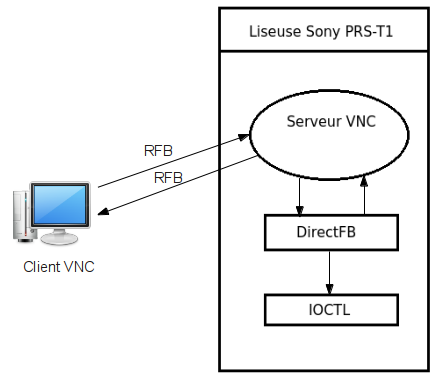
\includegraphics{VNCClientServeur.png}
\end{center}

\section{VNC et qemu}

Un autre point que l'on peut ajouter sur ce projet est d'intégrer VNC à qemu, cela afin que l'émulateur qemu puisse utiliser le serveur VNC installé sur la liseuse.


\section{Simulateur d'écran}

La dernière étape pour rendre le projet complet est de développer un simulateur d'écran de la liseuse. Pour cela il faut faire en sorte de gérer un affichage cohérent avec les temps de réponse de la liseuse Sony PRS-T1. C'est-à-dire que l'écran doit mettre un certain temps à se rafraîchir et pouvoir modifier seulement certaines zones de l'écran. De plus il faudrait y intégrer la gestion des événements, par exemple lors d'un clique souris simuler un appuie sur une zone de l'écran de la liseuse.

Enfin, une fois ce simulateur d'écran développé, l'objectif est de l'intégrer à qemu pour ne plus être dépendant de la liseuse. On aura alors un émulateur complet de la liseuse Sony PRS-T1.


%% A deplacer ...
\section{Protocol RFB}

RFB est un protocol simple pour l'accès à distance aux interfaces graphiques ds utilisateurs. C'est ce protocol qui est utilisé par VNC. Il y a d'un côté un visionneur, appelé client, et de l'autre côté un serveur qui va modifier le framebuffer afin de modifier l'affichage.

Le protocol RFB peut se décomposer en trois phases. Une première où le client et le serveur vont s'accorder sur la version du protocole à utiliser. Ensuite le client et le serveur vont s'envoyer des messages d'initialisation pour enfin pouvoir communiquer. A partir de ce moment, le client peut envoyer des demandes au serveur qui va lui retournera le résultat de cette requête.

\begin{center}
	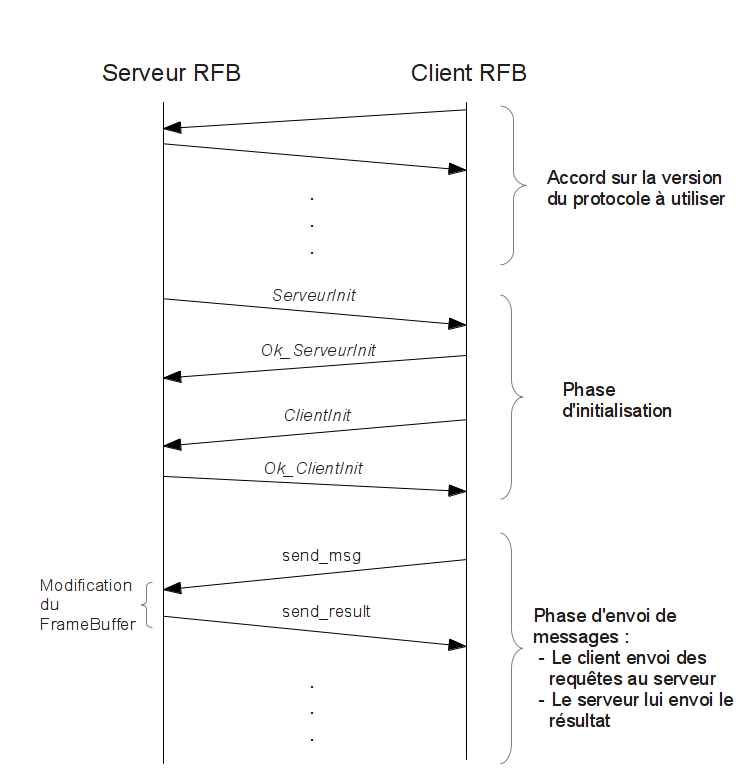
\includegraphics[scale=0.6]{RFBProtocol.png}
\end{center}
%\chapter{Bibliographie}

\bibliographystyle{plain} % Le style est mis entre accolades.
\bibliography{bibli} % mon fichier de base de données s'appelle bibli.bib
\nocite{ref1, ref2, ref3, ref4, ref5, ref6, ref7, ref8, ref9, ref10, ref11, ref12, ref13, ref14, ref15, ref16, ref17, ref18, ref19, ref20, ref21, ref22, ref23, ref24, ref25, ref26, ref27, ref28, ref29, ref30}

\end{document} 
